\documentclass{beamer}
\usepackage[hangul]{kotex}
\usepackage{graphicx}
\usepackage{href-ul}
\usetheme{Copenhagen}
\usecolortheme{beaver}
\usefonttheme{serif}
\SetHangulFonts{nanummj}{nanummj}{nanummj}

\definecolor{bgcolor}{RGB}{236, 220, 220}
\definecolor{fgcolor}{RGB}{190, 20, 20}
\setbeamercolor{title}{bg=bgcolor, fg=fgcolor}
\setbeamercolor{frametitle}{bg=bgcolor, fg=fgcolor}

\setbeamertemplate{section in toc}[circle]
\setbeamertemplate{subsection in toc}[square]
\setbeamertemplate{itemize items}[circle]
\setbeamertemplate{enumerate items}[circle]

\beamertemplateheadempty
\beamertemplatefootempty
\beamertemplatenavigationsymbolsempty

\newcommand{\spacing}{\hspace{0.3em}}
\newcommand{\eg}{\textbf{eg}}
\newcommand{\imgascii}{\textbf{img2ascii}}
\newcommand{\libpng}{\textbf{libpng}}
\newcommand{\Eigen}{\textbf{Eigen}}
\newcommand{\tonebased}{\textbf{tone-based}}
\newcommand{\structurebased}{\textbf{structure-based}}


\title{AAC - Ascii Art Converter}
\author{No More Double \\ 조다니엘, 박준영}
\date{\today}
\institute{Sogang University \\ CSE2035/AIE2051}

\begin{document}

\section{}
\begin{frame}{}
	\titlepage
	\begin{figure}
		\vspace{-1em}
		
\includegraphics[width=2cm]{sogang_university_logo}
		\vspace{1em}
	\end{figure}
\end{frame}

\section{}
\begin{frame}{}
	\frametitle{목차}
	\tableofcontents
\end{frame}

\section{왜 만들었는가?}
\begin{frame}{}
	\frametitle{왜 만들었는가?}
	\begin{itemize}
		\item AAC(악)이라는 이름이 너무 찰져서
		\item YouTube에서 donut.c라는 아스키 아트를 봤는데 멋있어서\footnote{\href{https://www.youtube.com/watch?v=DEqXNfs\_HhY}{\footnotesize{https://www.youtube.com/watch?v=DEqXNfs\_HhY}}}
	\end{itemize}
	\begin{figure}
		\centering
		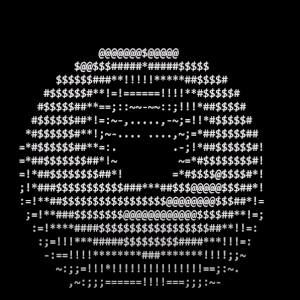
\includegraphics[width=4.5cm, height=4.5cm]{donut.png}
	\end{figure}
\end{frame}

\section{무엇으로 만들었는가?}
\begin{frame}{}
	\frametitle{무엇으로 만들었는가?}
	\begin{enumerate}
		\item 커스텀 라이브러리: \eg
		\item 메인 루틴: \imgascii
		\item 기타: GitHub, Valgrind, ...
	\end{enumerate}
\end{frame}

	\subsection{\eg}
	\begin{frame}{}
		\frametitle{\eg}
		\textbf{E}asypn\textbf{G}라는 뜻 \\
		\libpng \spacing + \Eigen으로 구성 \\
		이미지 입출력, 변환, 연산 등에 필요한 클래스를 내장
		\vspace{1em}
		\begin{itemize}
			\item egLoader: 이미지 입출력
			\item egMath: 변환에 필요한 연산
			\item egProcessing: 이미지 변환
			\item 등등... / egTypes나 egExceptions 같은 사소한 건 빼기
		\end{itemize}
	\end{frame}

	\subsection{\imgascii}
	\begin{frame}{}
		\frametitle{\imgascii}
		\eg \spacing 라이브러리를 활용하여 이미지를 처리하는 메인 루틴 \\
		\tonebased \spacing 방식과 \structurebased \spacing 방식으로 나뉨
		\begin{figure}
			(\tonebased \spacing 방식 결과물 사진 한 장, \structurebased \spacing 방식 결과물 사진 한 장 넣기)
		\end{figure}
	\end{frame}

	\subsection{기타}
	\begin{frame}{}
		\frametitle{기타}
		\begin{itemize}
			\item GitHub: 소스 코드 버전 관리 플랫폼
			\begin{figure}
				(Github 이미지 넣기)
			\end{figure}
			\item Valgrind: 메모리 누수 탐지 라이브러리
			\begin{figure}
				(Valgrind 메모리 누수 탐지 cmd창 이미지 넣기)
			\end{figure}
		\end{itemize}
	\end{frame}

\section{어떻게 동작하는가?}
\begin{frame}{}
	\frametitle{어떻게 동작하는가?}
	\begin{itemize}
		\item \tonebased \spacing 방식 - easy
		\item \structurebased \spacing 방식 - \underline{\textbf{EXTREMELY DIFFICULT}}
	\end{itemize}
\end{frame}

	\subsection{\tonebased \spacing 방식}
	\begin{frame}{}
		\frametitle{\tonebased \spacing 방식}
		\begin{enumerate}
			\item 이미지를 3차원 텐서 $ ( width, height, rgba ) $ 형태로 저장
			\item 각 픽셀별 red, green, blue 값의 평균을 구하여 밝기 도출
			\item 밝기 정보를 이용하여 이미지를 회색조로 변환
			\item 밝기에 해당하는 아스키 문자를 출력
		\end{enumerate}
	\end{frame}
	\begin{frame}
		\frametitle{결과}
		\begin{figure}
			\centering
			(처음 input 사진 한 장 $ \rightarrow $ 아스키 아트 사진 한 장)
		\end{figure}
	\end{frame}

	\subsection{\structurebased \spacing 방식}
	\begin{frame}{}
		\frametitle{\structurebased \spacing 방식}
		\begin{enumerate}
			\item 이미지를 3차원 텐서 $ ( width, height, rgba ) $ 형태로 저장
			\item 알고리즘 1 적용
			\item 알고리즘 2 적용
			\item 알고리즘 3 적용
			\item 알고리즘 4 적용
			\item 알고리즘 5 적용
			\item 알고리즘 6을 적용하여 아스키 문자를 선택
			\item 결과 출력
		\end{enumerate}
	\end{frame}
	\begin{frame}{}
		\frametitle{알고리즘 1}
		\begin{enumerate}
			\item 알고리즘 1 내용 설명 1 (1줄씩)
			\item 알고리즘 1 내용 설명 2 (1줄씩)
		\end{enumerate}	
		\begin{figure}
			(알고리즘 1로 이미지가 어떻게 변했는지 \\ before \& after 사진 넣기)
		\end{figure}
		(나머지 알고리즘도 이런 식으로 반복하면 될 듯)
	\end{frame}

% ---------------- 화이팅! ---------------- &

	\begin{frame}{}
		\frametitle{결과}
		\begin{figure}
			\centering
			(처음 input 사진 한 장 $ \rightarrow $ 아스키 아트 사진 한 장)
		\end{figure}
	\end{frame}

	\begin{frame}{}
		\frametitle{참고 자료}
		\begin{enumerate}
			\item 자료 1
			\item 자료 2
			\item 자료 3
		\end{enumerate}
		(인용 양식 지켜서 쓰면 교수님 호감 $ \rightarrow $ 대학원생으로 바로 납치)
	\end{frame}

	\begin{frame}
		\centering
		감사합니다.
	\end{frame}

\end{document}